Relate the values of momenta and their orientation to location on the Dalitz plot for the decay $p_0\to p_1+p_2+p_3$
using values indicated on the figures below.

\begin{center}
    \centering
    \begin{minipage}[c]{0.22\textwidth}
        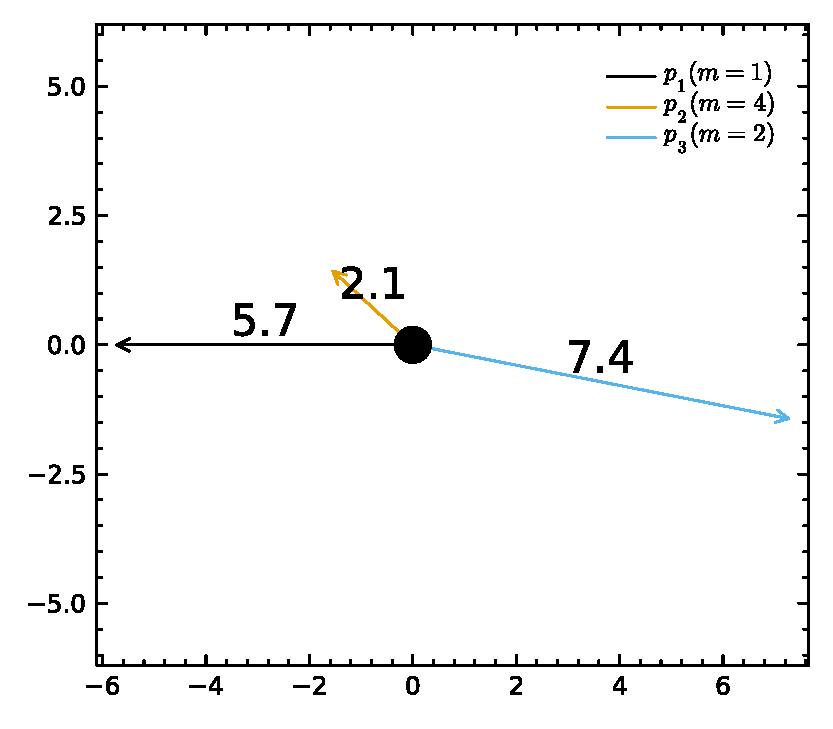
\includegraphics[width=\linewidth]{\figpath/four_momenta_1}
    \end{minipage}
    \hfill
    \begin{minipage}[c]{0.22\textwidth}
        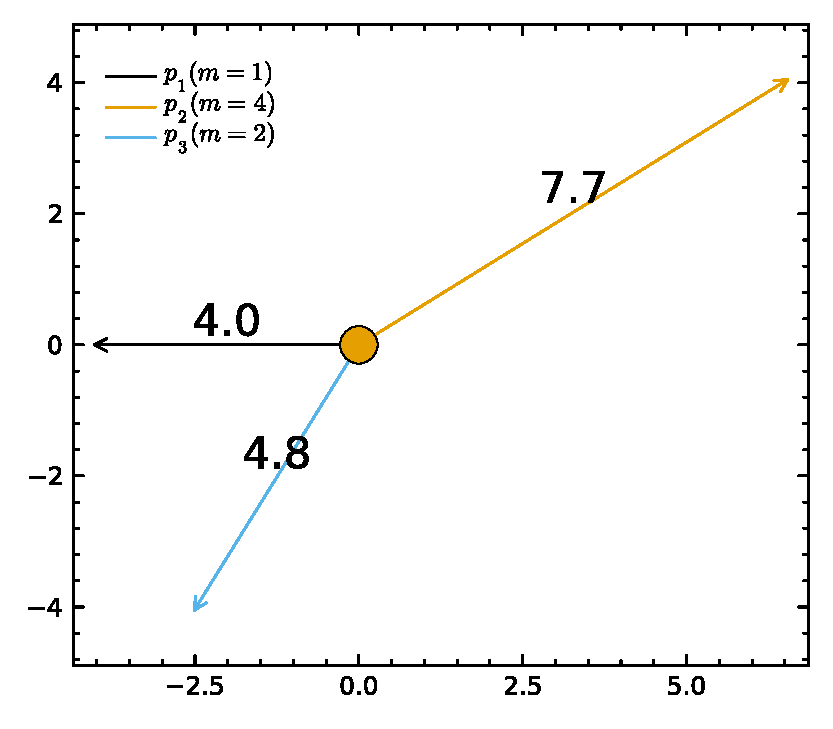
\includegraphics[width=\linewidth]{\figpath/four_momenta_2}
    \end{minipage}
    \hfill
    \begin{minipage}[c]{0.22\textwidth}
        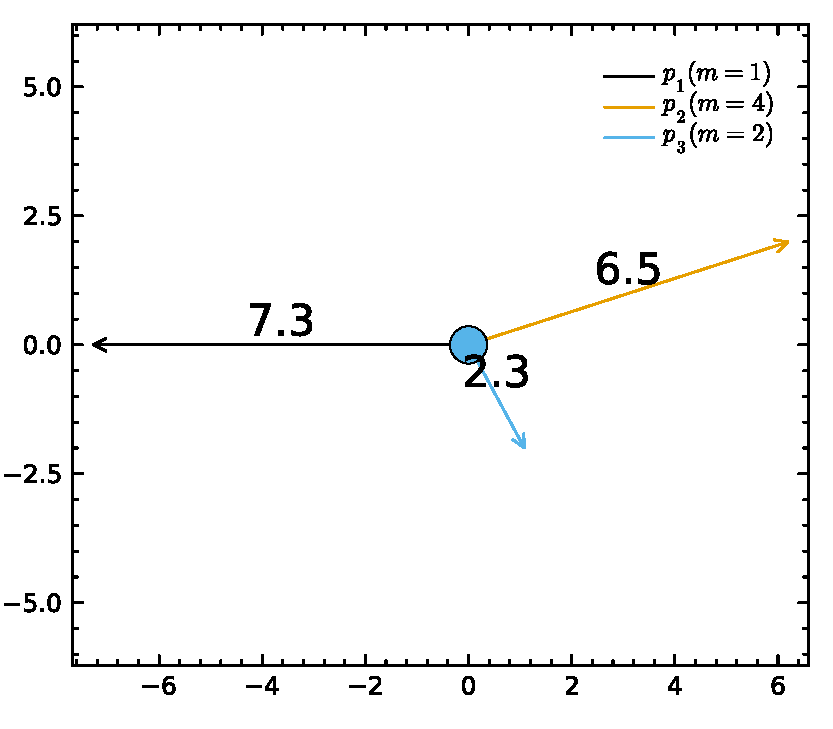
\includegraphics[width=\linewidth]{\figpath/four_momenta_3}
    \end{minipage}
    \hfill
    \begin{minipage}[c]{0.22\textwidth}
        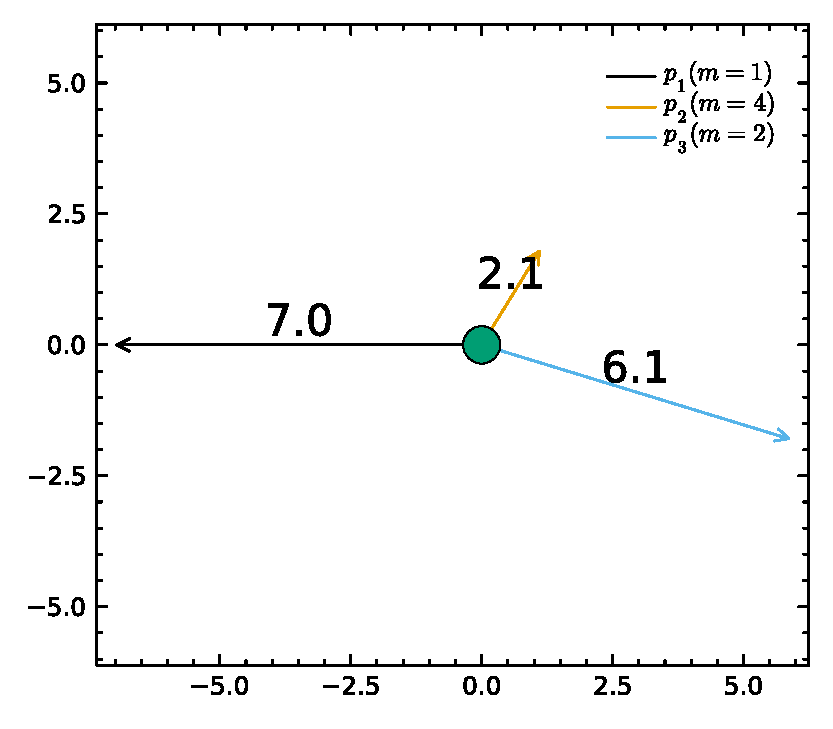
\includegraphics[width=\linewidth]{\figpath/four_momenta_4}
    \end{minipage}
    %   
    \begin{minipage}[c]{0.22\textwidth}
        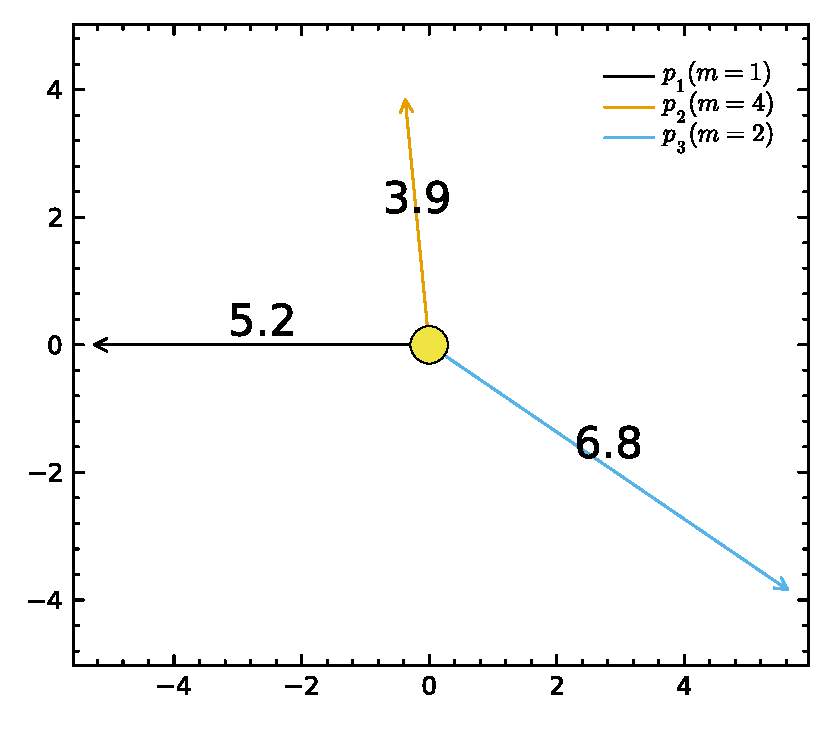
\includegraphics[width=\linewidth]{\figpath/four_momenta_5}
    \end{minipage}
    \hfill
    \begin{minipage}[c]{0.22\textwidth}
        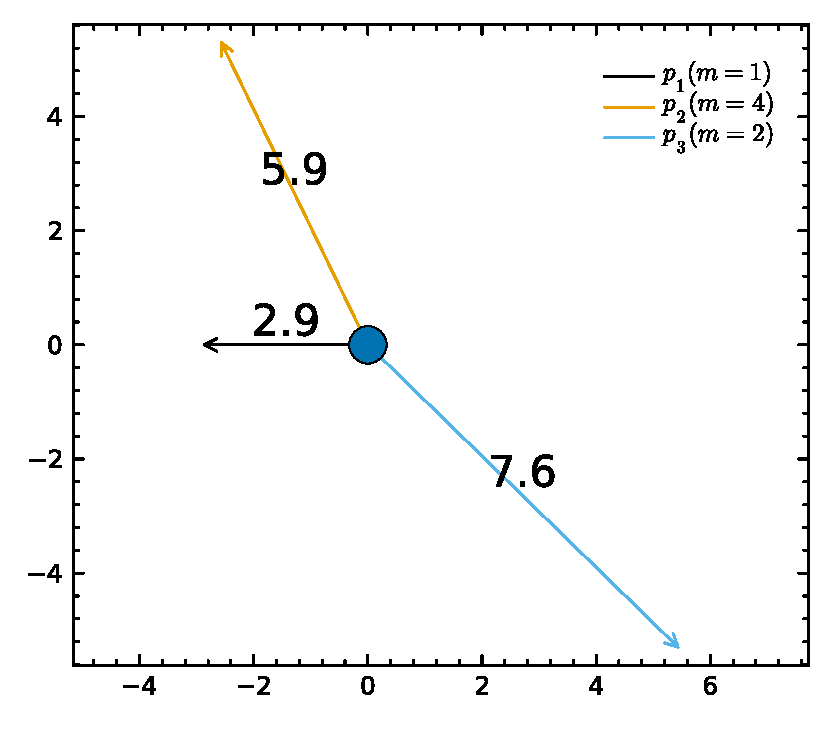
\includegraphics[width=\linewidth]{\figpath/four_momenta_6}
    \end{minipage}
    \hfill
    \begin{minipage}[c]{0.22\textwidth}
        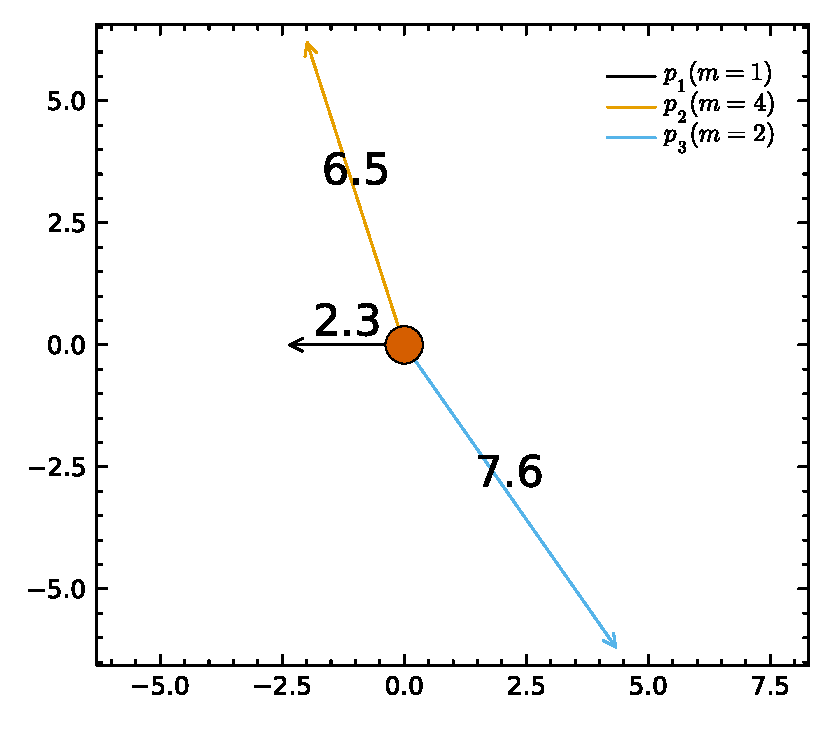
\includegraphics[width=\linewidth]{\figpath/four_momenta_7}
    \end{minipage}
    \hfill
    \begin{minipage}[c]{0.22\textwidth}
        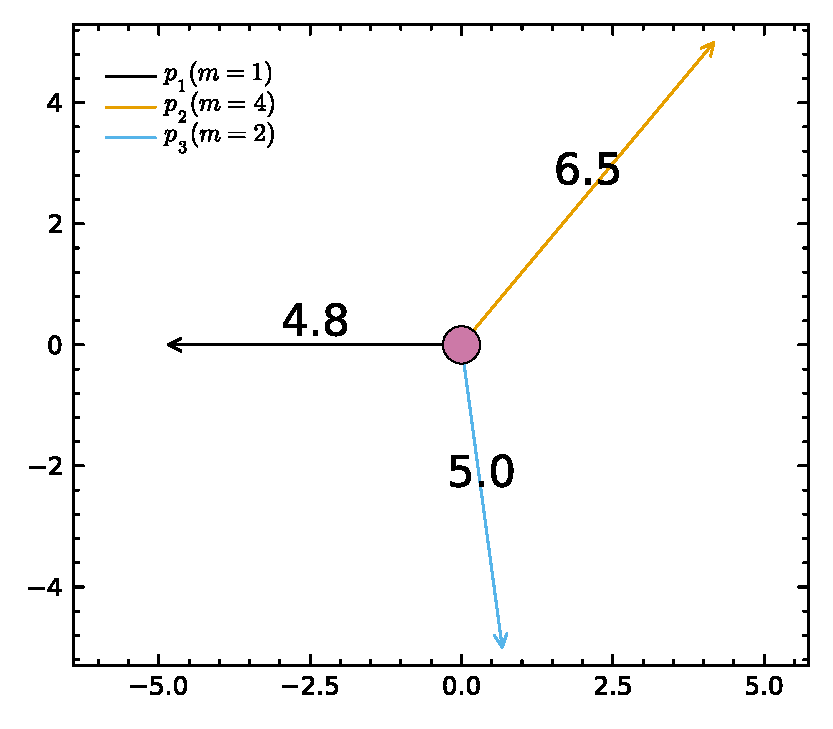
\includegraphics[width=\linewidth]{\figpath/four_momenta_8}
    \end{minipage}
\end{center}

\begin{solution}
    Mass is computed as
    \begin{align*}
        m_{ij} & = (p_i+p_j)^2 = m_i^2 + m_j^2 + 2 E_i E_j - 2p_i p_j \cos \angle \vec p_i \vec p_j\, \\
               & =m_i^2 + m_j^2 + 2 E_i E_j + p_i^2 + p_j^2 - p_k^2 \,                                \\
               & = (E_i + E_j)^2 - p_k^2
    \end{align*}
    the angle between the two momenta is traded to magnitude of momenta using algebra of three-vectors, $-\vec p_k = \vec p_i + \vec p_j $
    $$
        p_k^2  = p_i^2 + p_j^2 + 2 p_i p_j \cos \angle \vec p_i \vec p_j
    $$
    \fig{0.7}{four_momenta_solution}
\end{solution}
